\section{Evaluation}
\label{sect:results}
We first report on a study in which we evaluate the generation of distance candidates using the vector similarity measures and seed entities. 
We then discuss the results of five rounds of active learning using our ensemble of classifiers and our three sampling strategies: random, AL1 and AL2.
Finally, we experiment with word representations enhanced with character-level information using FastText~\cite{bojanowski2016enriching,joulin2016bag}.

\subsection{Dataset}
We work with a corpus composed of \nistnum{1690} full-text publications in HTML format downloaded from \textit{Macromolecules}, a relevant journal in polymer science.
These documents comprise \nistnum{381947} sentences and \nistnum{9229417} (\nistnum{253195} unique words or ``tokens'').
We set aside a test set of  100 documents with  \nistnum{22664} sentences and \nistnum{508391} (\nistnum{36293} unique) tokens. 
%\kyle{Prob should reverse this to instead describe the entire dataset and then the test set for initial training}\roselyne{done.}
We engaged six experts to identify one-word polymer names from our test set.
They extracted 467 unique one-word polymer names, which we use as gold standard.
When testing against this gold standard, we evaluate using a total of 9656 NLP-filtered nouns from the 100 documents.
We evaluate extraction accuracy in terms of precision and recall.
Recall refers to the fraction of actual positives that
are labeled correctly and precision to the fraction of predicted
positives that labeled correctly.

\subsection{Word Embedding Settings}
We explore how the choice of seed entities, the internal parameters \textit{vector} and \textit{window_size}  impact the number of target entities retrieved using similarity measures.
In order to estimate the entity-richness of our large pool of distance candidates and since we do not have manually extracted data for the entire corpus, we create a list of \nistnum{10000} distance candidate vectors most similar to our seed entity vectors and report the fraction of gold standard polymer extracted. 
Based on our experience of $\sim$ 5 polymers per document (\nistnum{8450} polymers for \nistnum{1690} documents), we can expect a fraction of the polymers found in the 100 gold standard documents to be extracted in the \nistnum{10000} candidates most similar to our seed entities.
We evaluate the entity-richness of polymers in this pool of candidates by measuring the percentage of the 467 manually extracted polymer names that it yields;
we use lower-case exact string matching between the gold standard polymer names and the proposed distance candidate strings to determine if a candidate is a polymer.
%\kyle{This text implies we know that there are 8450 polymers in our documents}
%\kyle{Are you trying to say by setting to 10K we are going well beyond what is likely to be polys? Given earlier
%we said there are 467 polys 10K is clearly a lot larger. Maybe better to frame this around the percentage of total tokens?}\roselyne{You got exactly what I was trying to say, 10k is a lot larger but it should also contain polys from the other papers, this number is just to "ensure" a certain percentage of our polys are in that pool. I'll try and rephrase.}

\subsubsection{Candidate Generation}
In previous work using the same corpus~\cite{tchoua2016hybrid,tchoua2016hybridi}, we build a dictionary of polymer names using a rule-based approach and aggregating synonyms across ChemDataExtractor records\textemdash a record consists of all information found about a chemical entity in a document.  
Having built this dictionary, we can identify the 10 most frequently occurring polymers in our corpus and their acronyms.
We assume that frequent polymers provide a large number of example sentences that illustrate context in which polymers are commonly used.
%\kyle{Might need to be more specific about what we use from our prior work. We can say we used a rule-based method and found the top N polymers?}
Hence, we first test the most common, the three most common and the ten most common polymers as seed entities.
We experiment with including and excluding their acronyms as corresponding additional seed entities.
(Note that this modest set of 1, 3 and 10 seed entities could also be suggested by an expert.)
Figure~\ref{fig:cand_generation1} shows the results for this set of experiments.
%\kyle{need to say how we determine if the results are polymers or not}\roselyne{fixed a little earlier}
%\kyle{might be clearer to state first that Polystytene gets to 35\%.. then by adding extra bits we can increase by XX etc.}
When using \textit{polystyrene} (the most commonly used name) as a seed entity, the pool of candidates contained 33.55 \% of the 467 gold standard polymers.
We note a 2 \% increase in the fraction of polymers retrieved when using \textit{polystyrene} and its acronym compared to using \textit{polystyrene} alone (37.69 \%).
The fraction of polymers increases by 10 \% when using the three most frequent polymers as seed entities (from 33.55 \% to 46.9 \% and 47.97 \% with acronyms). 
Using ten instead of three entities however, only slightly increases the yield of polymers by less than 1 \%, from 47.97 \% for three frequent polymers with acronyms to 48.39 \% for ten frequent polymers with acronyms.

In a second experiment, we further explore the idea of using multiple seed entities to increase the fraction of polymers retrieved in the pool of candidates.
We have built a small database of polymer properties ($\chi$DB) in previous work~\cite{choua2016hybrid,tchoua2016hybridi}. 
The $\chi$DB corpus included 111 our of 175 $\chi$DB polymers. 
We also scraped CrowDB, which lists some polymers and their properties at \url{http://polymerdatabase.com/} for polymer names.  
In this case, 32 out of 295 polymer names were found in our corpus.
We experiment using these 111 and 32 seed entities to extract polymers. The fraction of polymers from our gold standard is shown on Figure~\ref{fig:cand_generation2}.
These results confirm using more entities does not increase the yield of polymers, as some polymers have low frequency in the corpus, words that are most similar are less likely to be targets.

\kyle{perhaps better as a table. The long labels are hard to read}

\begin{figure*}
\centering
\begin{minipage}[b]{.4\textwidth}
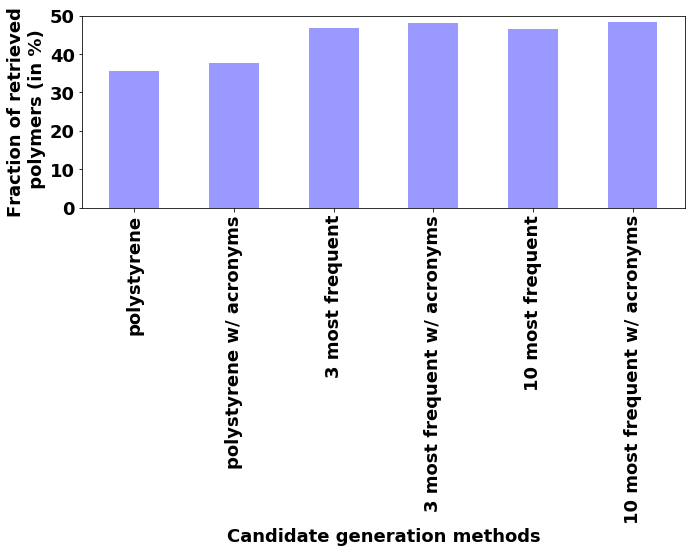
\includegraphics[trim=0in 0.1in 0.1in 0.in,clip,width=1.0\textwidth]{figures/candidate_generation_method1.png}
\caption{\label{fig:cand_generation1} Fraction of polymer retrieved for various candidate generation methods using most common, three most common and ten most common polymer names as seed entities.
}
\end{minipage}\qquad
\begin{minipage}[b]{.4\textwidth}
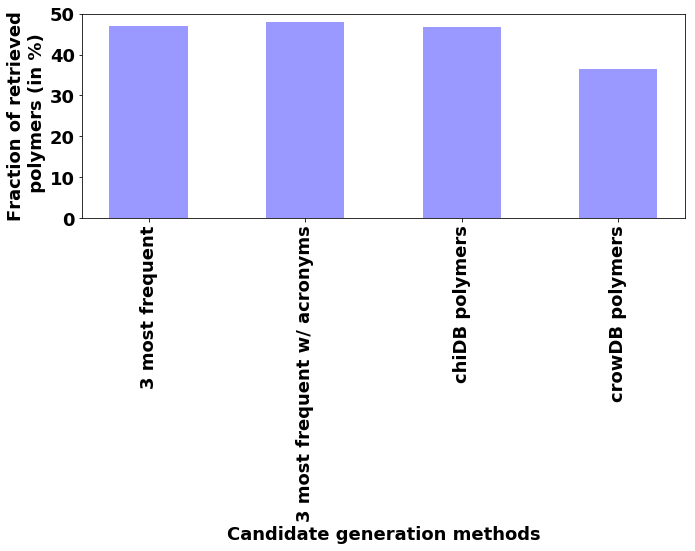
\includegraphics[trim=0in 0.1in 0.1in 0.in,clip,width=1.0\textwidth]{figures/candidate_generation_method2.png}
\caption{\label{fig:cand_generation2} Fraction of polymer retrieved for various candidate generation methods using three most common (with and without acronymss), $\chi$DB and CrowDB polymer names as seed entities.  \kyle{Not sure this needs to be a separate graph?}
}
\end{minipage}
\end{figure*}

%[35.55, 37.69, 46.9, 47.97, 46.47, 48.39]
%\begin{figure}[!t]
%\centering
%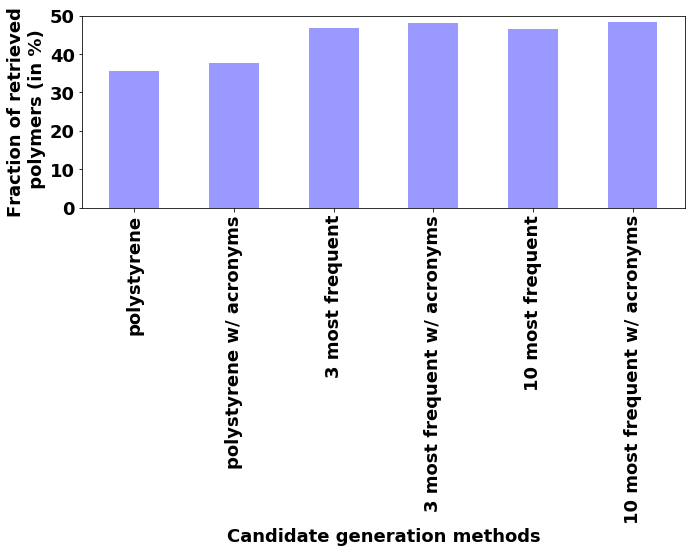
\includegraphics[trim=0in 0.1in 0.1in 0.in,clip,width=3.5in]{figures/candidate_generation_method1.png}
%\caption{\label{fig:cand_generation1} First set of experiments with seed entities showing noticeable improvement from 1 to 3 and less improvement from 3 to 10 seed entities.
%}
%\end{figure}
%[46.9, 47.97, 46.68, 36.4]
%\begin{figure}
%\centering
%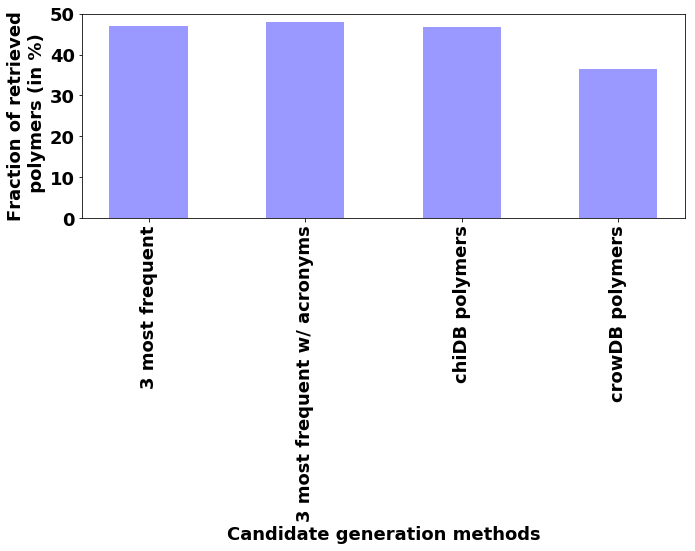
\includegraphics[trim=0in 0.1in 0.1in 0.in,clip,width=3.5in]{figures/candidate_generation_method2.png}
%\caption{\label{fig:cand_generation2} First set of experiments with seed entities showing that using more polymers as seed entities does not necessarily enrich the pool of distance candidates.
%}
%\end{figure}

\subsubsection{Tuning Parameters}
For the remainder of the experiments, we use the three most frequent polymers and their acronyms. 
We measure the impact of the \textit{window} and \textit{size} on the fraction of polymers extracted from the gold standard in the list of \nistnum{10000} candidates.
The \textit{window} represents the maximum distance between the current and predicted word within a sentence. In other words, it represents the number of words before and after each word considered by the neural network to generate a vector representation for that word. 
For each parameter setting, we measure the yield of polymers ten times for each window and vector size setting.
We observe slightly higher fraction of polymers retrieved for window sizes of 1 and 2. The yield subsequently decreases and more noticeably with window size larger than 5 (see Figure~\ref{fig:window_size}).
\kyle{Interesting that it is consistently decreasing. Except 8 seems to jump up. Any idea what the average sentence length is?}\roselyne{no but can find out, increase is not too noticeable though is it? still less than 4}
The \textit{size} simply determines the size of the word vector (features for our classifier)).
We varied this parameter between 100 and 500 and did not observe a maximum change of 1.05\% from the average fraction of polymers extracted (see Figure~\ref{fig:vector_size}). %\kyle{Maybe can say what the total difference was here}


\begin{figure*}
\centering
\begin{minipage}[b]{.4\textwidth}
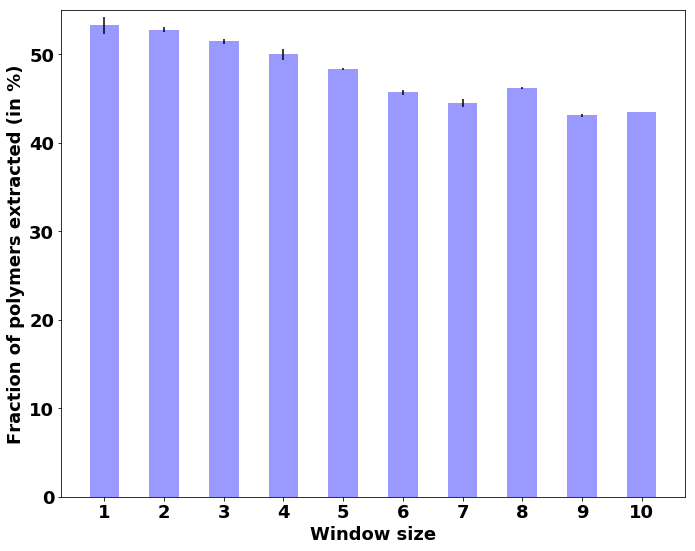
\includegraphics[trim=0in 0.1in 0.1in 0.in,clip,width=1.0\textwidth]{figures/window_size.png}
\caption{Impact of varying window size on fraction of polymers retrieved.}\label{fig:window_size}
\end{minipage}\qquad
\begin{minipage}[b]{.4\textwidth}
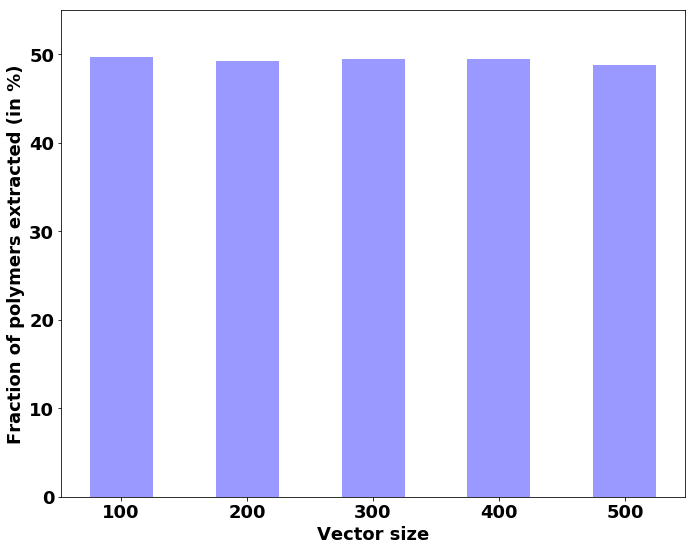
\includegraphics[trim=0in 0.1in 0.1in 0.in,clip,width=1.0\textwidth]{figures/vector_size.png}
\caption{Impact of varying vector size on fraction of polymers retrieved. \kyle{Not sure this fig is worth including}}\label{fig:vector_size}
\end{minipage}
\end{figure*}


%\begin{figure}[!t]
%\centering
%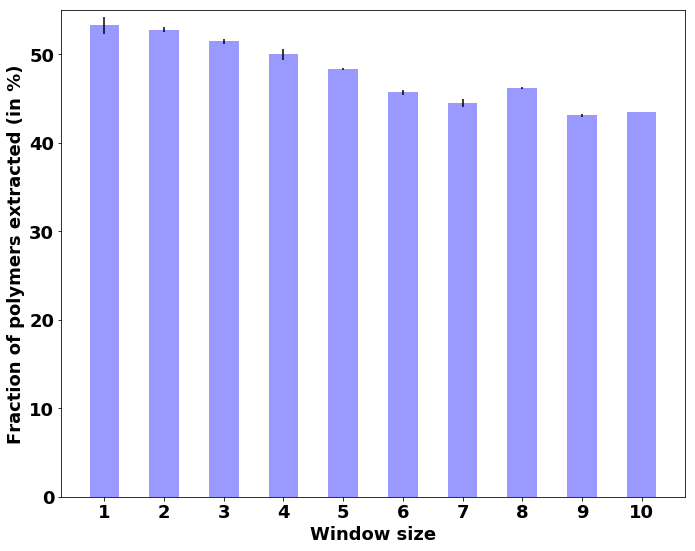
\includegraphics[trim=0in 0.1in 0.1in 0.in,clip,width=0.5\textwidth]{figures/window_size.png}
%\caption{\label{fig:window_size} Impact of varying window size on fraction of polymers retrieved.
%}

%\end{figure}
%[46.9, 47.97, 46.68, 36.4]
%\begin{figure}[!t]
%\centering
%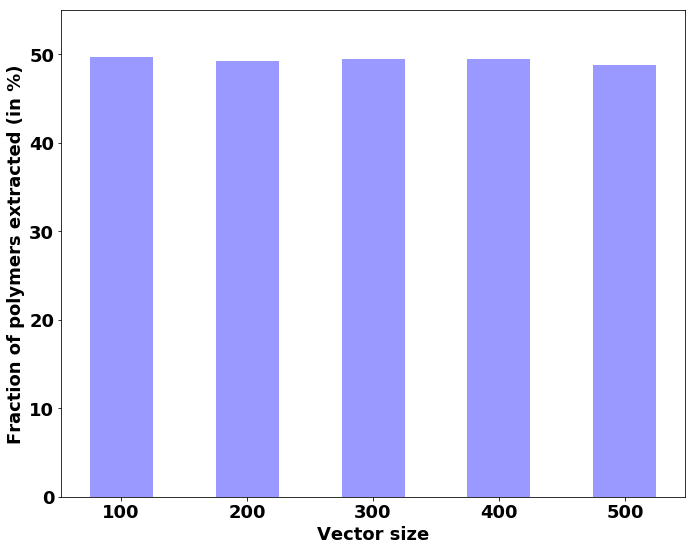
\includegraphics[trim=0in 0.1in 0.1in 0.in,clip,width=0.5\textwidth]{figures/vector_size.png}
%\caption{\label{fig:vector_size} Impact of varying vector size on fraction of polymers retrieved.
%}
%\end{figure}

\subsection{Active Learning}
Having explored the parameters for distance candidate generation, we generate a pool of \nistnum{10000} candidates most similar to the three most frequent polymers and their acronyms from a test corpus of \nistnum{1590} (this time excluding our 100 gold standard documents). 
The candidates are arranged in decreasing order of similarity scores and we use a window size of 2 and a vector size of 200.  

\subsubsection{Initial Classifier}
In order to blance the initial training set (increase the potential number of target entities),
we initially train the classifier using the first
200 entities from the above mentioned list of \nistnum{10000}.
%\kyle{Don't completely understand previous sentence}\roselyne{Hopefully cleared this out above}
Recall that the batch size of 200 was set based on an estimate of 30-60 minutes of expert time.
As described on Figure~\ref{fig:current}, in the first step, we train and test on candidates generated from a word embedding model generated using only the training documents. 
We update the word embedding model to include the 100 documents from which experts extracted our gold standard polymer names and retrain multiple classifiers, before testing the best performing classifier on all NLP-filtered nouns from the 100 test documents.
Figure~\ref{fig:roc_init} shows the Receiver Operating Curve (ROC) for the initial classifier with highest recall when evaluating on the test corpus. 
The ROC plot is an evaluation measure that is based on two basic evaluation measures: specificity (true positive rate) and sensitivity (true negative rate).
Sensitivity is the same as recall. Specificity is a measure of the true negative rate (the proportion of actual negatives that are correctly identified as such).
A classifier with the random performance level always has the same 0.5 true positive rate and false negative rate.
A classifier with the perfect performance level shows a combination of two straight lines immediately showing a true positive rate of 1.0 and remaining there as recall increases.
Classifiers with meaningful performance levels usually lie in the area between the random ROC curve (baseline) and the perfect ROC curve. 
The area under the curve (AUC) measures the area under the ROC.
Ideally the AUC of a learning algorithm is above 0.5. 
Since AUC takes into account true negatives or correctly predicted non-polymers and our dataset is imbalanced containing more non-polymers than polymers, we also plot the Precision Recall Curve (PRC) to visualize the tradeoff between precision and recall.

While the AUC for the initial base KNN classifier is above random performance in Figure~\ref{fig:roc_init}, the initial PRC shows poor precision regardless of recall (see Figure~\ref{fig:prc_init}).
In this round of labeling KNN is selected as the model with best recall in all three steps of Figure~\ref{fig:current}.\\

\begin{figure*}
\centering
\begin{minipage}[b]{.4\textwidth}
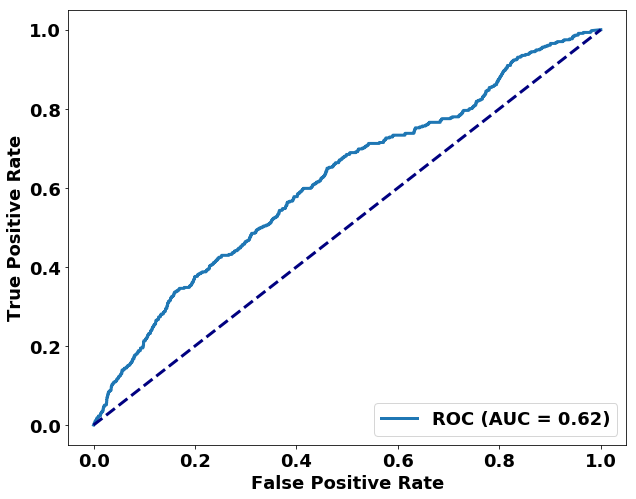
\includegraphics[trim=0in 0.1in 0.1in 0.in,clip,width=1.0\textwidth]{figures/roc_init.png}
\caption{Receiver Operating Curve for KNN model for initial round of labels.}\label{fig:roc_init}
\end{minipage}\qquad
\begin{minipage}[b]{.4\textwidth}
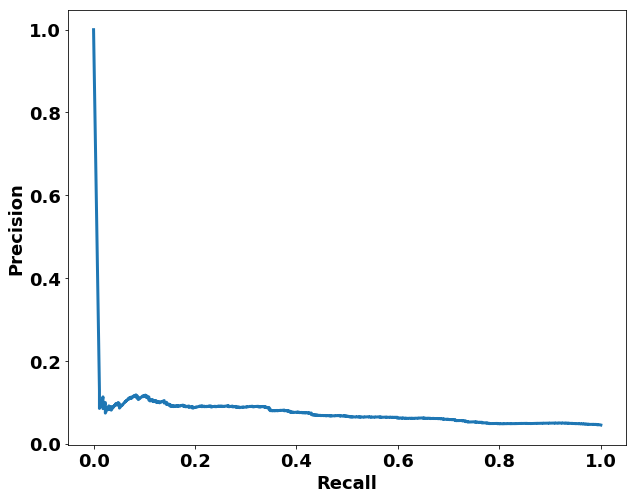
\includegraphics[trim=0in 0.1in 0.1in 0.in,clip,width=1.0\textwidth]{figures/prc_init.png}
\caption{Precision Recall Curve for KNN model for initial round of labels.}\label{fig:prc_init}
\end{minipage}
%\end{figure*}

%\begin{figure*}
\centering
\begin{minipage}[b]{.4\textwidth}
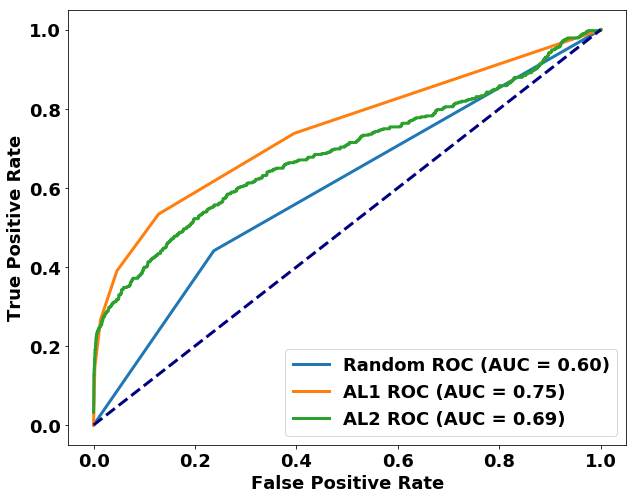
\includegraphics[trim=0in 0.1in 0.1in 0.in,clip,width=1.0\textwidth]{figures/rocs_round4.png}
\captionsetup{labelformat=empty}
\caption{Receiver Operating Curve for iteration 3.}\label{fig:roc_round4}
\end{minipage}\qquad
\begin{minipage}[b]{.4\textwidth}
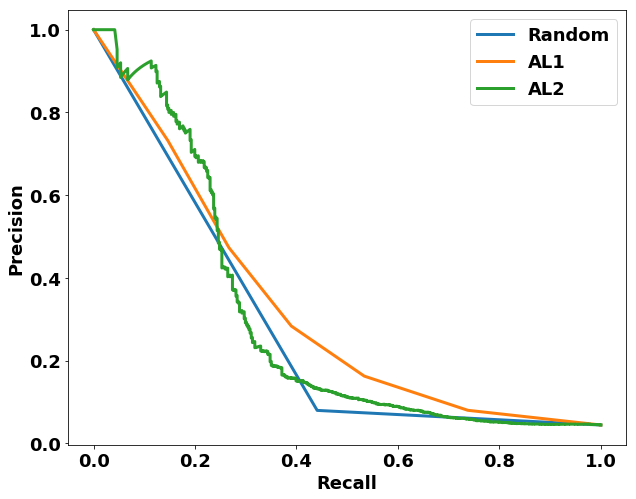
\includegraphics[trim=0in 0.1in 0.1in 0.in,clip,width=1.0\textwidth]{figures/prcs_round4.png}
\captionsetup{labelformat=empty}
\caption{Precision Recall Curves for iteration 3.}\label{fig:prcs_round4}
\end{minipage}

\centering
\begin{minipage}[b]{.4\textwidth}
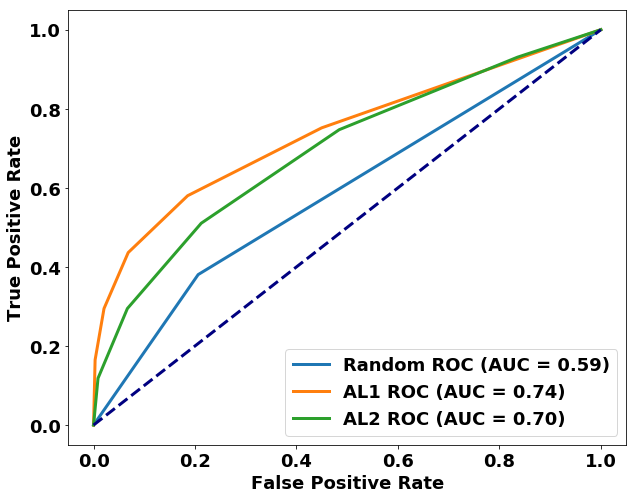
\includegraphics[trim=0in 0.1in 0.1in 0.in,clip,width=1.0\textwidth]{figures/rocs_round5.png}
\captionsetup{labelformat=empty}
\caption{Receiver Operating Curve for iteration 4.}\label{fig:rocs_round5}
\end{minipage}\qquad
\begin{minipage}[b]{.4\textwidth}
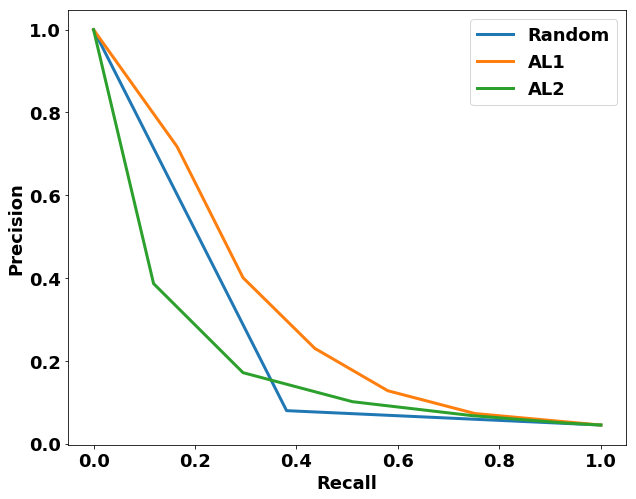
\includegraphics[trim=0in 0.1in 0.1in 0.in,clip,width=1.0\textwidth]{figures/prcs_round5.png}
\captionsetup{labelformat=empty}
\caption{Precision Recall Curves for iteration 4.}\label{fig:prcs_round5}
\end{minipage}
\setcounter{figure}{8}  
\caption{Receiver Operation and Precision Recall Curves for iterations 4 and 5. AL - 1 refers to active learning using NLP-filtered nouns. AL - 2 refers to active learning using candidates deemed similar to seed entities.}\label{fig:rocs_prcs_round5}
\end{figure*}

\subsubsection{Discrimination Phase}
After the first round, we experiment with the three strategies mentioned in \S\ref{sect:architecture}: random sampling (Random), active learning using pool of NLP-filtered nouns from training corpus (AL1), and active learning using pool of \nistnum{10000} distance candidates deemed closest to our seed entities(AL2) \textemdash minus 200 used in initial round).
Given the relatively small batch size, we see no improvement for two rounds of active learning or first three rounds of labeling. 
Precision remains under 6\% across all used classifiers. 
Another sign of poor performance was the inconsistency of classifier choices across active learning iterations, 
as well as in steps 1, 2 and 3 of Figure~\ref{fig:current}.
However in the third iteration of active learning, we notice an increase in precision across strategies as shown in Figure~\ref{fig:rocs_prcs_round5} and a more consistent choice of classifiers.
By the fourth iteration of active learning, the random strategy still does not show signs of learning. 
The selected decision tree classifier has only learned two probabilities and the precision for higher recall remains close to random sampling ($\sim 6\%$).
This learning is sustained in the following iteration as illustrated on Figures~\ref{fig:rocs_prcs_round5}. 
The AUC for AL1 is 0.74 and that of AL2 is 0.70. The PRCs are improved over the first round with AL1 showing better tradeoff than AL2 and Random.\\

%\kyle{what does it look like if we put all iterations for a particular method on one graph}\roselyne{terrible and I don't think we should do this because it highlights that we were trying different algorithms and saving classifiers that maybe can't be directly compared to each other. Also, it just all looks random}.
%\kyle{IF we went beyond 5 rounds do you think performance would continue to improve? Or is it leveling off?}\roselyne{I think it should improve. We stop here because we detect learning and we now have "enough" labels. Or we stop here because we've used 4 hours of expert time for each strategy or 8 total... either way, this is enough to reach CDE with all labels.}

At this point we observe predictive ability and combine all labels (from the three strategies: Random, AL1 and AL2 for a total of 2542 labels) for training a KNN classifier (most frequently selected classifier during the active learning phase).
We test NLP-filtered nouns from our 100-document test set.
While Figure~\ref{fig:all_rocs} shows an AUC of 0.74 and Figure~\ref{fig:all_prcs} shows an improved precision-recall curve, precision is generally low.
When tested against our gold standard of 467 one-word polymer names the KNN classifier achieves 25.0\% precision and  42.5\% recall.	
It is worth noting that with limited training data and based solely on context, the classifiers retreives more than one third of the gold standard polymers with a precision of one in four candidates being a polymer; this after about ten hours of expert labeleing.

\begin{figure*}
\centering
\begin{minipage}[b]{.4\textwidth}
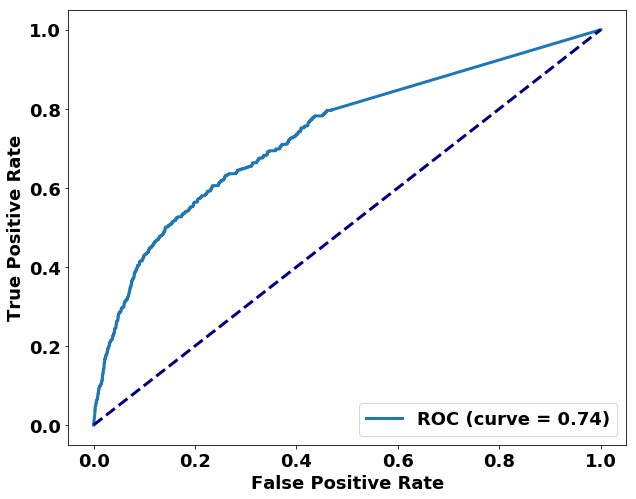
\includegraphics[trim=0in 0.1in 0.1in 0.in,clip,width=1.0\textwidth]{figures/roc_all_gensim.png}
\caption{Receiver Operating Curve for KNN model trained using all annotated labels.}\label{fig:all_rocs}
\end{minipage}\qquad
\begin{minipage}[b]{.4\textwidth}
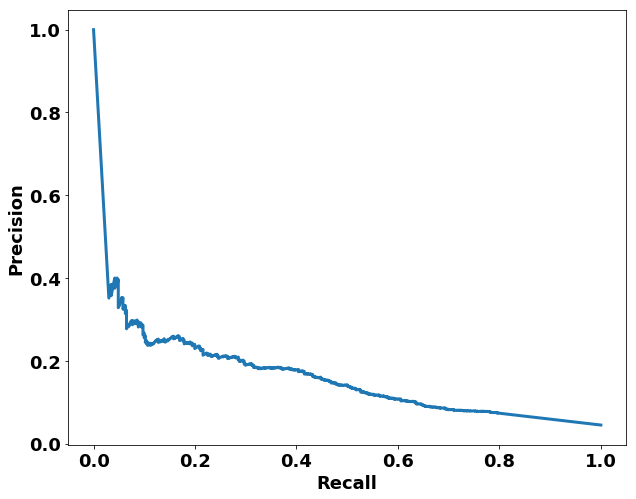
\includegraphics[trim=0in 0.1in 0.1in 0.in,clip,width=1.0\textwidth]{figures/prc_all_gensim.png}
\caption{Precision Recall Curve for KNN model trained using all annotated labels.}\label{fig:all_prcs}
\end{minipage}
\end{figure*}


\subsection{Using polyNER's labels}
Next, we train a different word embedding model using polyNER's labels.
FastText uses word representations enriched with character-level information using FastText.
This word embedding method considers sub-word information as well as
context, allowing it to consider word morphology differences, such as prefixes
and suffixes. Sub-word information is especially useful for words for which
context information is lacking, as words can still be compared to morphologically similar
existing words. We set the length of the sub-word used for comparison\textemdash
FastText's n_gram parameter\textemdash to five characters, based on our intuition that
many polymers begin with the prefixes ``poly'' or ``poly(.'' \\

Therefore, we generate a FastText word embedding mode, and use our labeled candidates to train this different word vectors enhanced with character level information.
Once again, we train a KNN classifier using all labels (generated through all 3 strategies)
 and test NLP-filtered nouns from our 100-document test set.
The KNN classifier performance improves when using these word vectors as shown in Figures~\ref{fig:all_rocs_fasttext} and~\ref{fig:all_prcs_fasttext}.
In this case, the classifier achieves 31.7\% precision and 82.3\% recall. 
These numbers are comparable to those achieved by ChemDataExtractor (CDE), a state-of-the-art chemical NLP tool.
As CDE aims to extract all
chemical compounds, not just polymers, it serves only as a demonstration of an
alternative approach in the absence of a polymer NER system (Note that CDE also extracts properties). 
Its recall is high
at 74.5\% but its precision is, as expected, low at 8.7\%. 
We have previously enhanced CDE with
manually defined polymer identification rules~\cite{tchoua2017towards},
and our polymer-enhanced version of the software (CDE+) achieved 42.2\% precision and 68.3\% recall on the same test set. 
We achieve higher recall in both cases and intermediate precision with only $\sim$ ten hours of expert labeling including an hour of completing untrained users' reviews of randomly sampled candidates.

\begin{figure*}
\centering
\begin{minipage}[b]{.4\textwidth}
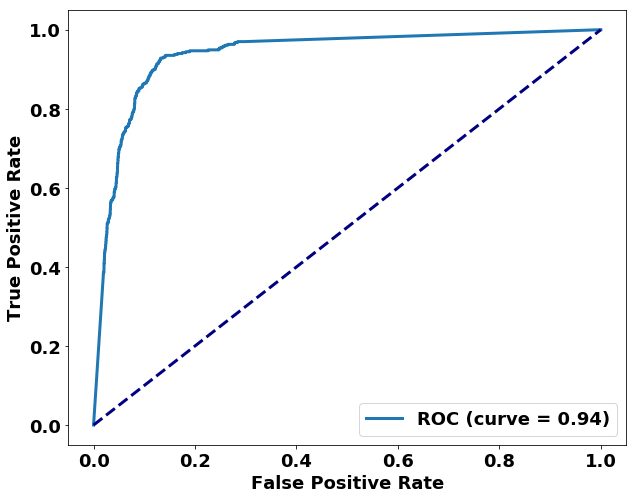
\includegraphics[trim=0in 0.1in 0.1in 0.in,clip,width=1.0\textwidth]{figures/roc_all.png}
\caption{Receiver Operating Curve for KNN model trained using all annotated labels and word representations enriched with character-level information.}\label{fig:all_rocs_fasttext}
\end{minipage}\qquad
\begin{minipage}[b]{.4\textwidth}
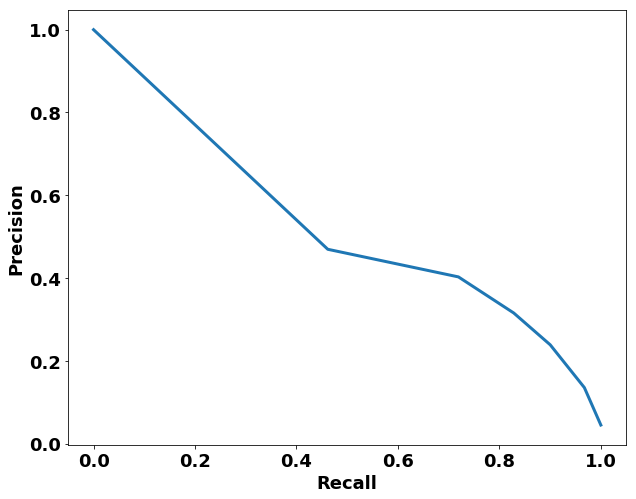
\includegraphics[trim=0in 0.1in 0.1in 0.in,clip,width=1.0\textwidth]{figures/prc_all.png}
\caption{Precision Recall Curve for KNN model trained using all annnotated labels and word representations enriched with character-level information.}\label{fig:all_prcs_fasttext}
\end{minipage}
\end{figure*}






